\documentclass[10pt, twocolumn, twoside, letterpaper]{IEEEtran}

\usepackage[activate={true, nocompatibility}, final, tracking=true, kerning=true, spacing=true, factor=1100, stretch=10, shrink=10]{microtype}
\linespread{0.9}

%\def\mycopyrightnotice{
%  {\footnotesize
%  \begin{minipage}{\textwidth}
%  \centering
%  {978-1-7281-4164-0/19/\$31.00 \copyright2019 IEEE
%  \end{minipage}
%  }
%}

\makeatletter
\def\ps@IEEEtitlepagestyle{
  %\def\@oddfoot{\mycopyrightnotice}
  \def\@evenfoot{}
}

\ifCLASSINFOpdf
   \usepackage[pdftex]{graphicx}
\else
   \usepackage[dvips]{graphicx}
\fi

\ifCLASSOPTIONcompsoc
  \usepackage[caption=false, font=normalsize, labelfont=sf, textfont=sf]{subfig}
\else
  \usepackage[caption=false, font=footnotesize]{subfig}
\fi

\usepackage{amsmath}
\usepackage{bm}
\usepackage{amssymb}
\usepackage{algorithm}
\usepackage{algorithmic}
\usepackage{stfloats}
\usepackage{url}
\usepackage{siunitx}
\usepackage{fancyref}
\usepackage{textgreek}

\usepackage[acronym, nomain]{glossaries}

% Define "long-s" key: 
\glsaddkey* {longs}% key 
{\glsentrylong{\glslabel}s}% default value 
{\glsentrylongs}% command analogous to \glsentrytext 
{\Glsentrylongs}% command analogous to \Glsentrytext 
{\glslongs}% command analogous to \glstext 
{\Glslongs}% command analogous to \Glstext 
{\GLSlongs}% command analogous to \GLStext

%% Define "short-s" key: 
\glsaddkey* {shorts}% key 
{\glsentryshort{\glslabel}s}% default value 
{\glsentryshorts}% command analogous to \glsentrytext 
{\Glsentryshorts}% command analogous to \Glsentrytext 
{\glsshorts}% command analogous to \glstext 
{\Glsshorts}% command analogous to \Glstext 
{\GLSshorts}% command analogous to \GLStext

\DeclareRobustCommand{\glss}[1]
{%
  \ifglsused{#1}{\glsshorts{#1}}{\glslongs{#1} (\glsshorts{#1})\glsunset{#1}}%
}

\DeclareRobustCommand{\Glss}[1]
{%
  \ifglsused{#1}{\Glsshorts{#1}}{\Glslongs{#1} (\glsshorts{#1})\glsunset{#1}}%
}

\newacronym{1D}{1D}{$1$-Dimensional}
\newacronym{2D}{2D}{$2$-Dimensional}
\newacronym{3D}{3D}{$3$-Dimensional}
\newacronym[longs={$3$-Dimensional Point Clouds}, shorts={3DPCs}]{3DPC}{3DPC}{$3$-Dimensional Point Cloud}
\newacronym{4D}{4D}{$4$-Dimensional}
\newacronym{4DCT}{4DCT}{$4$-Dimensional Computed Tomography}
\newacronym[longs={Attenuation Corrections}, shorts={ACs}]{AC}{AC}{Attenuation Corrected}
\newacronym[longs={Affine Deformations}, shorts={ADs}]{AD}{AD}{Affine Deformation}
\newacronym{AP}{AP}{Anterior Posterior}
\newacronym{ATP}{ATP}{Adenosine Triphosphate}
\newacronym[longs={B-Splines}, shorts={BSs}]{BS}{BS}{B-Spline}
\newacronym[longs={Cross Correlations}, shorts={CCs}]{CC}{CC}{Cross Correlation}
\newacronym{CCT}{CCT}{Cine Computed Tomography}
\newacronym{CG}{CG}{Conjugate Gradient}
\newacronym{COM}{COM}{Centre of Mass}
\newacronym[longs={Control Points}, shorts={CPs}]{CP}{CP}{Control Point}
\newacronym[longs={Control Point Grids}, shorts={CPGs}]{CPG}{CPG}{Control Point Grid}
\newacronym{CT}{CT}{Computed Tomography}
\newacronym{DD}{DD}{Data Driven}
\newacronym{DDG}{DDG}{Data Driven Gating}
\newacronym[longs={Deformation Vector Fields}, shorts={DVFs}]{DVF}{DVF}{Deformation Vector Field}
\newacronym{EANM}{EANM}{European Association of Nuclear Medicine}
\newacronym{EM}{EM}{Expectation Maximisation}
\newacronym{FDG}{FDG}{Fluorodeoxyglucose}
\newacronym{F-FDG}{F-FDG}{Fluorine-$18$ Fludeoxyglucose}
\newacronym[longs={Fields of View}, shorts={FOVs}]{FOV}{FOV}{Field Of View}
\newacronym{FWHM}{FWHM}{Full Width at Half Maximum}
\newacronym{GD}{GD}{Gradient Descent}
\newacronym{GE}{GE}{General Electric}
\newacronym[longs={Ground Truths}, shorts={GTs}]{GT}{GT}{Ground Truth}
\newacronym{HU}{HU}{Hounsfield Unit}
\newacronym[longs={Image Registrations}, shorts={IRs}]{IR}{IR}{Image Registration}
\newacronym{KBq/mL}{KBq/mL}{Kilo Becquerel per Millilitre}
\newacronym{KeV}{KeV}{Kilo Electron Volt}
\newacronym{KV}{KV}{Kilo Volt}
\newacronym[longs={Light Emitting Diodes}, shorts={LEDs}]{LED}{LED}{Light Emitting Diode}
\newacronym[longs={Lines of Responses}, shorts={LORs}]{LOR}{LOR}{Line of Response}
\newacronym[longs={Mean Absolute Errors}, shorts={MAEs}]{MAE}{MAE}{Mean Absolute Error}
\newacronym{MAPE}{MAPE}{Mean Absolute Percentage Error}
\newacronym{MBF}{MBF}{Myocardial Blood Flow}
\newacronym[longs={Motion Compensated Images}, shorts={MCIs}]{MCI}{MCI}{Motion Compensated Image}
\newacronym{MC}{MC}{Motion Corrected}
\newacronym{MI}{MI}{Mutual Information}
\newacronym{ML}{ML}{Maximum Likelihood}
\newacronym{MLAA}{MLAA}{Maximum Likelihood Reconstruction of Activity and Attenuation}
\newacronym{MLE}{MLE}{Maximum Likelihood Estimation}
\newacronym{MLEM}{MLEM}{Maximum Likelihood Expectation Maximisation}
\newacronym[longs={Motion Models}, shorts={MMs}]{MM}{MM}{Motion Model}
\newacronym[longs={Myocardial Perfusion Images}, shorts={MPIs}]{MPI}{MPI}{Myocardial Perfusion Imaging}
\newacronym{MR}{MR}{Magnetic Resonance}
\newacronym{MSE}{MSE}{Mean Squared Error}
\newacronym[longs={Attenuation Maps}, shorts={Mu-Maps}]{Mu-Map}{Mu-Map}{Attenuation Map}
\newacronym[longs={Non-Attenuation Corrections}, shorts={NACs}]{NAC}{NAC}{Non-Attenuation Corrected}
\newacronym{NMI}{NMI}{Normalised Mutual Information}
\newacronym{ND}{ND}{$n$-Dimensional}
\newacronym[longs={Non-Rigid Deformations}]{NRD}{NRD}{Non-Rigid Deformation}
\newacronym{nonTOF}{nonTOF}{Non-Time-of-Flight}
\newacronym{OSEM}{OSEM}{Ordered Subset Expectation Maximisation}
\newacronym[longs={Principal Components}, shorts={PCs}]{PC}{PC}{Principal Component}
\newacronym{PCA}{PCA}{Principal Component Analysis}
\newacronym{PET}{PET}{Positron Emission Tomography}
\newacronym{PSMA}{PSMA}{Prostate Specific Membrane Antigen}
\newacronym[longs={Respiratory Correspondence Models}, shorts={RCMs}]{RCM}{RCM}{Respiratory Correspondence Model}
\newacronym[longs={Rigid Deformations}, shorts={RDs}]{RD}{RD}{Rigid Deformation}
\newacronym{RDP}{RDP}{Relative Difference Prior}
\newacronym{RM}{RM}{Respiratory Motion}
\newacronym[longs={Regions of Interest}, shorts={ROIs}]{ROI}{ROI}{Region of Interest}
\newacronym{RPM}{RPM}{Real Time Position Management}
\newacronym{SGD}{SGD}{Stochastic Gradient Descent}
\newacronym{SI}{SI}{Superior Inferior}
\newacronym{SIRF}{SIRF}{Synergistic Image Reconstruction Framework}
\newacronym[longs={Signal to Noise Ratios}, shorts={SNRs}]{SNR}{SNR}{Signal to Noise Ratio}
\newacronym[longs={Surrogate Signals}, shorts={SSs}]{SS}{SS}{Surrogate Signal}
\newacronym{SSD}{SSD}{Sum of Squared Differences}
\newacronym{STIR}{STIR}{Software for Tomographic Image Reconstruction}
\newacronym[longs={Standard Uptake Values}, shorts={SUVs}]{SUV}{SUV}{Standard Uptake Value}
\newacronym{SVD}{SVD}{Singular Value Decomposition}
\newacronym{TOF}{TOF}{Time-of-Flight}
\newacronym[longs={Thin Plate Splines}, shorts={TPSs}]{TPS}{TPS}{Thin Plate Spline}
\newacronym{XCAT}{XCAT}{$4$-Dimensional Extended Cardiac Torso}


\newcommand{\cmmnt}[1]{\@bsphack\@esphack}

\usepackage[style=ieee, doi=false, isbn=false, url=false, maxbibnames=1, minbibnames=1, maxcitenames=1, mincitenames=1, backend=biber, defernumbers=false]{biblatex}
\addbibresource{./bibtex/bib/Biblio.bib}

%\IEEEpubid{\begin{minipage}{\textwidth}\ \\[9pt] \centering
%\medskip
%\\
%978-1-7281-2260-1/19/\$31.00~\copyright~2019~IEEE
%\end{minipage}}

\begin{document}
\title{PET/CT Respiratory Motion Correction With a Single Attenuation Map Using NAC Derived Deformation Fields}

\pagestyle{plain}
\pagenumbering{gobble}

\author{Alexander~C.~Whitehead,~\IEEEmembership{Student~Member,~IEEE,}
        Ander~Biguri,
        Nikos~Efthimiou,~\IEEEmembership{Member~IEEE},
        Scott~W.~Wollenweber,~\IEEEmembership{Senior~Member~IEEE,}
        Charles~W.~Stearns,~\IEEEmembership{Fellow,~IEEE,}
        Brian~F.~Hutton,~\IEEEmembership{Senior~Member,~IEEE,}
        Jamie~R.~McClelland
        and~Kris~Thielemans,~\IEEEmembership{Senior~Member,~IEEE}%

    \thanks{Alexander~C.~Whitehead, Ander~Biguri, Brian~F.~Hutton \& Kris~Thielemans are with the Institute of Nuclear Medicine, University College London, London, NW1~2BU, UK (contact: \texttt{alexander.whitehead.18@ucl.ac.uk}).}%
    \thanks{Nikos~Efthimiou is with the Department Radiology, Perelman School of Medicine, University of Pennsylvania, Philadelphia, PA 19104-6055, USA.}%
    \thanks{Alexander~C.~Whitehead \& Jamie~R.~McClelland are with the Centre for Medical Image Computing, University College London, London, NW1~2BU, UK.}%
    \thanks{Scott~Wollenweber \& Charles~Stearns are with Molecular Imaging \& Computed Tomography Engineering, GE Healthcare, USA}%
    \thanks{This research is supported by GE Healthcare, the NIHR UCLH Biomedical Research Centre \& the EPSRC-funded UCL Centre for Doctoral Training in Medical Imaging (EP/L016478/1). The software used was partly produced by the Computational Collaborative Project in Synergistic PET-MR Reconstruction, CCP PET-MR, UK EPSRC grant EP/M022587/1 \& the CCP on Synergistic Biomedical Imaging, CCP SyneRBI, UK EPSRC grant EP/T026693/1}%
    \thanks{Jamie~R.~McClelland is supported by a Cancer Research UK Centres Network Accelerator Award Grant (A21993) to the ART-NET consortium \& a CRUK Multi-disciplinary grant (CRC 521).}%
}

\maketitle
\IEEEpeerreviewmaketitle

\begin{abstract}
    Respiratory motion correction is beneficial in positron emission tomography. Different strategies for handling attenuation correction exist. In clinical practice, usually a single attenuation map is available, derived from CT in one respiratory state. This can introduce an unwanted bias (through misaligned anatomy) into the motion correction algorithm. This paper builds upon previous work which suggested that non-attenuation corrected data was suitable for motion correction, through the use of motion models, if time of flight data are available. Here, the previous work is expanded upon by incorporating attenuation correction in an iterative process. The proposed method can handle variations in intra- \& inter-cycle motion. Non-attenuation corrected volumes are reconstructed using ordered subset expectation maximisation \& used as input for motion model estimation. A single attenuation map is then warped to the volumes, using the motion model, \& the volumes are attenuation corrected, after which another motion estimation \& correction cycle is performed. For validation, XCAT simulations are used, for one bed position, with a field of view including the base of the lungs \& the diaphragm. The output from the proposed method is evaluated against a non-motion corrected reconstruction of the same data using both a visual \& standardised uptake value analysis as well as a profiles volume. Results indicate that  motion correction of inter-respiratory cycle motion is possible with this method, while accounting for attenuation deformation. The implications for future research include the possibility of directly incorporating the motion model estimation into the reconstruction algorithm as well as also attempting to simultaneously estimate deformations for the attenuation map as well as the activity distribution.
\end{abstract}

\section{Introduction} \label{sec:introduction}
    \IEEEPARstart{R}{espiratory} motion reduces image resolution in \gls{PET} by introducing blurring and mis-alignment artefacts~\cite{Nehmeh2008a}. Unless gated \gls{CT} are available (which themselves increase dose to the patient), to avoid mis-registration due to attenuation mismatches, most existing \gls{MC} methods rely on pair-wise registration of gated \gls{NAC} \gls{PET} volumes~\cite{LungMotionDiaphragmBaiBib}.%~\cite{Oliveira2014}.
    This is a challenging problem due to the low contrast and high noise of these volumes. Other \gls{MC} methods can incorporate, directly, both \gls{MC} and \glss{Mu-Map} estimation into reconstruction, however, these can be computationally expensive~\cite{Bousse2016b}.
    
    In our previous work we investigated the possibility of using \gls{MM} for respiratory \gls{MC} where the \gls{RCM} was derived from \gls{NAC} \gls{PET}. One of the advantages of using a \gls{MM} approach over pair-wise registering the data is that by incorporating a fit of the \gls{DVF} to the \gls{SS}, noise is diminished. We found that \gls{NAC} \gls{TOF} \gls{PET} was suitable to estimate the motion from gated PET data without inter-respiratory cycle variation~\cite{Whitehead2019ImpactPET}. This work extends the method towards attenuation correction with a single \gls{Mu-Map} (from any position).

\vspace{-0.5cm}

\section{Methods} \label{sec:methods}
    \subsection{XCAT Volume Generation} \label{sec:xcat_volume_generation}
        \gls{XCAT}%~\cite{Segars2010} 
        was used to generate $240$ volumes over a \SI{120}{\second} respiratory trace (with inter-respiratory cycle variation) derived from a data captured using a \gls{RPM}. The max displacement of \gls{AP} and \gls{SI} motion was set to \SI{1.2}{\centi\metre} and \SI{2.0}{\centi\metre} respectively. Activity concentrations were derived from a static \gls{FDG} patient scan. The \gls{FOV} included the base of the lungs, diaphragm and the top of the liver with a \SI{20}{\milli\metre} diameter spherical lesion placed into the centre of the right lung.
    
    \vspace{-0.5cm}
    
    \subsection{PET Acquisition Simulation} \label{sec:pet_acquisition_simulation}
        \gls{PET} acquisitions were simulated %(and reconstructed)
        using \gls{STIR}~\cite{Thielemans2012, Efthimiou2018} through the \gls{SIRF}~\cite{Ovtchinnikov2019CCPPETMRSIRF} to forward project the data using the geometry of a \gls{GE} Discovery $710$ with a \gls{TOF} resolution of \SI{375}{\pico\second}. This \gls{TOF} resolution is higher than that of the $710$, but is closer to the newer \gls{GE} Signa PET/MR system. \gls{TOF} mashing was used to reduce computation time resulting in $13$ \gls{TOF} time bins of size \SI{376.5}{\pico\second}. Attenuation was included using the relevant \glss{Mu-Map} generated by \gls{XCAT}. Scatter and randoms were not taken into account. Multiple noise realisations were generated to simulate an acquisition over \SI{120}{\second}, emulating a standard single bed position acquisition. A respiratory \gls{SS} was generated using \gls{PCA}~\cite{Thielemans2011}.
        This was used to gate the data into $10$ respiratory bins using displacement gating.% For the purpose of the \gls{RCM} fitting, \gls{SS} values were ascertained for the post-gated data by taking an average of the \gls{SS} values of the data in each bin.
    
    \vspace{-0.5cm}
    
    \subsection{Non-Attenuation Corrected Image Reconstruction} \label{sec:non-attenuation_corrected_image_reconstruction}
        Data were reconstructed without \gls{AC} using \gls{OSEM} with two full iterations and $24$ subsets.%~\cite{Hudson1994}.
        Volumes were post-filtered using a Gaussian blur with a kernel size of \SI{6.4}{\milli\metre} \gls{FWHM}.
    
    \vspace{-0.5cm}
    
    \subsection{Motion Model Estimation} \label{sec:motion_model_estimation}
        The \gls{MM} method used in this work uses \gls{3D} B-spline \glss{CPG} with the corresponding warping operation denoted as $\mathbf{W}(\mathbf{\alpha}_t)$, with $\mathbf{\alpha}_t$ a vector with coefficients at time $t$ and the breathing surrogate signal $\mathbf{s}$:
    
        \vspace{-0.25cm}
        
        \begin{equation}
            \forall t \in [1, n_t],\quad \alpha_{k, t} := R_{1, k} s_{1, t} + R_{2, k}
        \end{equation}
        
        \vspace{-0.025cm}
        
        \noindent where $\alpha_{k, t}$ is the coefficient for node $k$ at time point $t$, and $R_{i, k}$ are the model parameters where $i = [1, 2]$~\cite{McClelland2017}. A generalised framework unifying \gls{IR} and respiratory \glss{MM} was used to estimate \glss{RCM} and \glss{MCI}~\cite{McClelland2017}. \gls{SSD} was used as the similarity measure and bending energy was used as a penalty.% The \gls{CPG} spacing and penalty weight were tuned using a grid search.
    
    \vspace{-0.5cm}
    
    \subsection{Attenuation Map Warping} \label{sec:attenuation_map_warping}
        A \gls{Mu-Map} close to the mean respiratory position was selected from the \glss{Mu-Map} generated by \gls{XCAT}, this \gls{Mu-Map} was then registered (using \gls{NMI}) to the mean position NAC volume generated from the \gls{RCM}.
        The \gls{RCM} was then used to generate \glss{DVF} for the \gls{SS} values of each bin, which were then used to warp the \gls{Mu-Map} from the mean respiratory position to each bin.
    
    \vspace{-0.5cm}
    
    \subsection{Motion Corrected Image Reconstruction with AC} \label{sec:attenuation_corrected_image_reconstruction}
        Data were re-reconstructed with \gls{AC} using the \glss{Mu-Map} from~\Fref{sec:attenuation_map_warping}. The same reconstruction parameters as in~\Fref{sec:attenuation_corrected_image_reconstruction} were used. This data was then either motion correction using the original \gls{NAC} \gls{RCM} or a new \gls{RCM} was fit on the \gls{AC} volumes as in~\Fref{sec:motion_model_estimation}.
    
    \vspace{-0.5cm}
    
    \subsection{Evaluation} \label{sec:evaluation}
        %To evaluate the validity of the \gls{MM} results, the \gls{COM} of the lesion, over time, was tracked for both \gls{NAC} and \gls{AC} reconstructions. This was achieved by warping a volume only including the lesion in the reference position, and then computing its \gls{COM}.
        
        In addition to the reconstructions performed in~\Fref{sec:attenuation_corrected_image_reconstruction} data were also reconstructed after simply summing all gates together,  using either a sum of all \glss{Mu-Map} (to emulate an average CINE-CT) or one \gls{Mu-Map}, positioned  close to the mean respiratory position. This process matches clinical practise . 
        
        Comparisons used included: A profile over the lesion and \gls{SUV}\textsubscript{max}, \gls{SUV}\textsubscript{median} and \gls{SUV}\textsubscript{peak}. \gls{SUV}\textsubscript{peak} here was defined following \gls{EANM} guidelines.%~\cite{Boellaard2015FDG2.0}

\vspace{-0.5cm}

\section{Results} \label{sec:results}
    %\begin{figure}
    %    \centering
    %    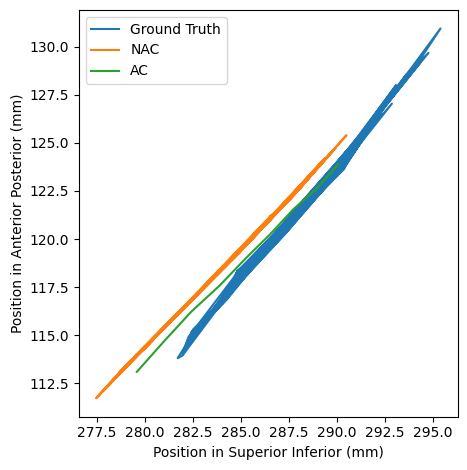
\includegraphics[width=0.5\linewidth]{figures/com.png}
    %    \captionsetup{singlelinecheck=false, justification=centering}
    %    \caption{The path of the \gls{COM} of the lesion. Horizontal (respectively vertical) axis corresponds to motion in the \gls{SI} (respectively \gls{AP}). Different curves denote \gls{COM} displacement for  ground truth data, the estimated data from the \gls{NAC} based \gls{RCM} and the estimated data from the \gls{AC} based \gls{RCM}.}
    %    \label{fig:com}
    %\end{figure}
    
    %\gls{COM} results can be seen in~\Fref{fig:com}, the \gls{COM} of both the \gls{NAC} and \gls{AC} matches closely the ground truth \gls{COM}.
    
    \begin{figure}
        \vspace{-0.5cm}
        \centering
        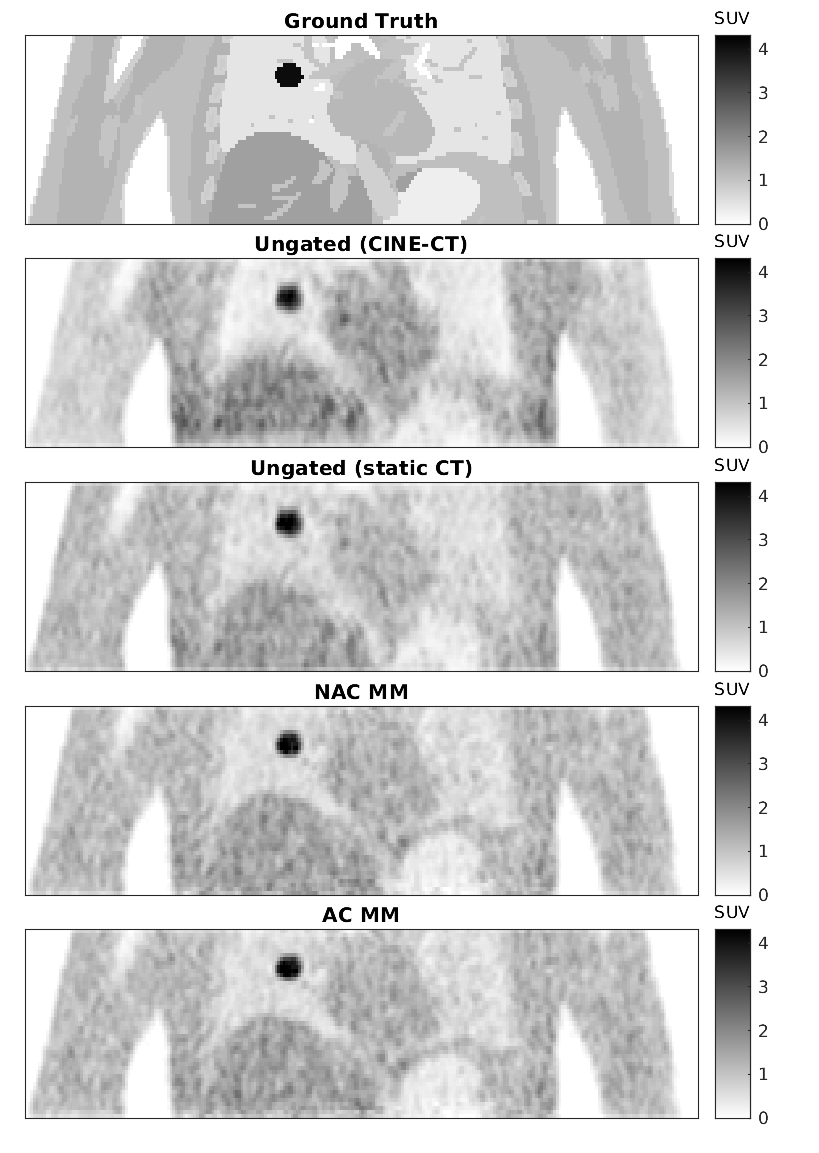
\includegraphics[width=0.9\linewidth]{figures/visual_analysis.png}
        \captionsetup{singlelinecheck=false, justification=centering}
        \caption{Reconstructions using; ungated (CINE-\gls{CT}), ungated (static \gls{CT}), \gls{NAC} \gls{MM}, \gls{AC} \gls{MM}. Colour map ranges are consistent for all images.}
        \label{fig:visual_analysis}
        \vspace{-0.5cm}
    \end{figure}
    
    \begin{figure}
        \vspace{-0.0cm}
        \centering
        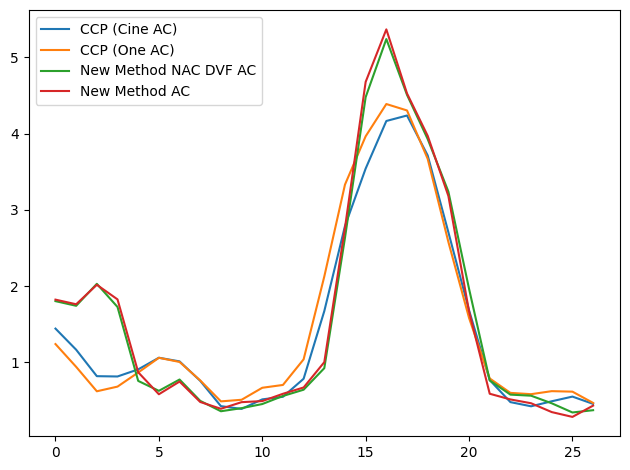
\includegraphics[width=1.0\linewidth]{figures/profile.png}
        \captionsetup{singlelinecheck=false, justification=centering}
        \caption{A profile across the lesion for; ungated (CINE-\gls{CT}), ungated (static \gls{CT}), \gls{NAC} \gls{MM}, \gls{AC} \gls{MM}.}
        \label{fig:profile}
        \vspace{-0.5cm}
    \end{figure}
    
    \begin{table}
        \vspace{-0.5cm}
        \centering
        \captionsetup{singlelinecheck=false, justification=centering}
        \caption{Comparison of \gls{SUV}\textsubscript{max}, \gls{SUV}\textsubscript{median} and \gls{SUV}\textsubscript{peak} between; ungated (CINE-\gls{CT}), ungated (static \gls{CT}), \gls{NAC} \gls{MM}, \gls{AC} \gls{MM}.}
        
        \resizebox*{1.0\linewidth}{!}
        {
            \begin{tabular}{||c|ccc||}
                \hline
                \textbf{\gls{SUV}} & \textbf{Max} & \textbf{Median} & \textbf{Peak} \\
                \hline
                \textbf{Ungated (CINE-\gls{CT})}    & $4.63$ & $2.73$ & $3.39$ \\
                \textbf{Ungated (static \gls{CT})}  & $4.66$ & $3.05$ & $3.54$ \\
                \hline
                \textbf{\gls{NAC} \gls{MM}}         & $5.56$ & $3.18$ & $4.07$ \\
                \textbf{\gls{AC} \gls{MM}}          & $5.43$ & $3.18$ & $4.00$ \\
                \hline
            \end{tabular}
        }
        \label{tab:suv}
        \vspace{-0.5cm}
    \end{table}
    
     The ungated and the \gls{MM} data can be seen in~\Fref{fig:visual_analysis}. When compared visually structures can be seen, less blurred, in the \gls{MM} data that cannot be seen in the ungated data, for instance, structures at the boundary between the diaphragm and the lung. Additionally the lesion itself can be seen to be more homogeneous, this can be observed in the profile across the lesion in~\Fref{fig:profile}. \gls{SUV} results can be seen in~\Fref{tab:suv} and consistently show that \glss{SUV} are greater for the \gls{MM} over ungated method.

\vspace{-0.5cm}

\section{Discussion and Conclusions} \label{sec:discussion_and_conclusions}
    Results from both a visual analysis, a comparison of profiles and \glss{SUV} show that the \gls{MM} provides volumes more free from blurring and less susceptible to artefacts when compared to the ungated data.
    %
    In the future, we will incorporate the estimated \glss{DVF} into the reconstruction. We will also compare  more complex methods of combining  motion estimation and image reconstruction based on \cite{Bousse2016b}.
    

\AtNextBibliography{\scriptsize}
\printbibliography

\end{document}
